\documentclass[11pt]{article}

\usepackage[margin=1in]{geometry}
\usepackage{amsmath,amssymb}
\usepackage{booktabs}
\usepackage{graphicx}
\usepackage{float}
\usepackage{hyperref}
\usepackage{enumitem}
\usepackage{xcolor}

\graphicspath{{../../../phase_01_python_prototype/figures/}}

\title{Phase 1 Report: DOA-Sector Inference with LIF-Inspired Edge Processing}
\author{Hossein Molhem\\Kennesaw State University\\EE 6900 Embedded AI}
\date{\today}

\begin{document}
\maketitle

\begin{abstract}
This report documents Phase 1 of an embedded-AI project focused on lightweight spike-based inference for edge sensing. A complete Python reference prototype was developed for direction-of-arrival (DOA) sector classification using a physics-based uniform linear array (ULA) signal model. The processing chain includes covariance estimation, beamspace feature extraction, feature normalization, nearest-centroid baseline classification, rate-based spike encoding, and leaky-integrate-and-fire (LIF)-inspired temporal inference. The nearest-centroid baseline achieved an overall test accuracy of $0.869048$. A fixed LIF configuration achieved $0.825000$ accuracy with a mean stable-decision latency of $6.423810$ time steps. A later LIF parameter sweep improved the best LIF accuracy to $0.841667$ at $T=40$ and leak $=0.99$. These results demonstrate a clear and controllable accuracy--latency trade-off, which is central to the embedded AI motivation of the project.
\end{abstract}

\tableofcontents
\newpage

\section{Purpose and Scope}

The purpose of Phase 1 is to establish a complete and reproducible Python reference model for DOA-sector inference using a physics-based sensing model and a hardware-aware spike-based inference path. This phase is not intended to introduce a new high-resolution DOA algorithm. Instead, it provides an engineering baseline that can later be refactored toward embedded execution, PYNQ deployment, or Vitis HLS acceleration.

The completed prototype connects three technical layers:

\begin{enumerate}[label=\arabic*.]
    \item array signal processing through a ULA signal model and covariance-derived beamspace features,
    \item machine-learning baseline evaluation through nearest-centroid classification,
    \item sparse temporal inference through rate-based spike encoding and LIF-inspired evidence accumulation.
\end{enumerate}

\section{Theoretical Background}

This section summarizes the theoretical foundation used in Phase 1. The purpose is to keep the main report self-contained while avoiding unnecessary derivation detail in the main body. Additional mathematical details are provided in the Appendix.

\subsection{Uniform Linear Array Signal Model}

A uniform linear array consists of $N$ equally spaced sensor elements. For a narrowband plane wave arriving from angle $\theta$, the relative phase progression across the array is determined by the element spacing $d$, the wavelength $\lambda$, and the wavenumber $k=2\pi/\lambda$. With a broadside angle convention, a typical ULA steering vector can be written as
\begin{equation}
    a(\theta)
    =
    \begin{bmatrix}
    1 & e^{-jkd\sin\theta} & e^{-j2kd\sin\theta} & \cdots & e^{-j(N-1)kd\sin\theta}
    \end{bmatrix}^{T}.
\end{equation}
For the Phase 1 prototype, the exact objective is not continuous-angle estimation. Instead, the steering-vector model is used to generate physically meaningful array snapshots for a four-sector DOA classification task.

\subsection{Sample Covariance Matrix}

For each simulated source angle and SNR value, the received snapshot matrix is modeled as
\begin{equation}
    X = a(\theta)s + N,
\end{equation}
where $a(\theta)$ is the steering vector, $s$ is the source waveform, and $N$ is additive complex noise. The sample covariance matrix is
\begin{equation}
    R_{xx}=\frac{1}{M}XX^{H},
\end{equation}
where $M$ is the number of snapshots. In expectation, the covariance structure contains spatial information through the rank-one signal component associated with $a(\theta)a^{H}(\theta)$ and a noise contribution determined by the SNR.

\subsection{Beamspace Feature Extraction}

Beamspace processing maps array-domain information into a set of angular responses. For a steering vector $b(\phi)$ evaluated at grid angle $\phi$, a simple beamspace energy feature can be represented as
\begin{equation}
    p(\phi)=b^{H}(\phi)R_{xx}b(\phi).
\end{equation}
Evaluating $p(\phi)$ on a fixed angular grid produces a compact real-valued feature vector. In Phase 1, this feature vector is used for coarse sector classification rather than fine DOA estimation.

\subsection{Nearest-Centroid Classification}

The non-spiking baseline uses a nearest-centroid decision rule. If $x$ is a normalized feature vector and $\mu_c$ is the training-set centroid for class $c$, the baseline decision is
\begin{equation}
    \hat{c}=\arg\min_{c}\|x-\mu_c\|_2^2.
\end{equation}
This classifier is intentionally simple and interpretable. It provides a useful reference for measuring how much accuracy is lost when continuous-valued features are converted into sparse spike trains.

\subsection{Rate-Based Spike Encoding}

After normalization, each feature component is mapped to a spike probability. For feature component $z_i \in [0,1]$, the spike at time step $t$ can be modeled as
\begin{equation}
    s_i[t] \sim \mathrm{Bernoulli}(z_i).
\end{equation}
The time-average spike count approximates the original normalized feature value:
\begin{equation}
    \mathbb{E}\left[\frac{1}{T}\sum_{t=1}^{T}s_i[t]\right]=z_i.
\end{equation}
This representation introduces stochastic quantization error but creates a sparse temporal signal appropriate for hardware-facing inference experiments.

\subsection{LIF-Inspired Temporal Inference}

The LIF-inspired classifier accumulates spike-driven evidence over time. For class $c$, the membrane evidence follows
\begin{equation}
    v_c[t]=\alpha v_c[t-1]+i_c[t],
\end{equation}
where $\alpha$ is the leak factor and $i_c[t]$ is the spike-driven input current. A higher leak value preserves past evidence more strongly, while a shorter time window reduces latency but may reduce classification accuracy.

\subsection{Stable-Decision Latency}

The classifier produces a class decision at each time step by selecting the largest membrane value:
\begin{equation}
    d[t]=\arg\max_{c}v_c[t].
\end{equation}
The stable-decision latency is defined as the earliest time step after which the decision remains equal to the final decision. This metric provides a practical way to evaluate whether the temporal classifier can support early-exit or adaptive-latency edge inference.

\section{Signal Model and Dataset}

The Phase 1 dataset is generated using a narrowband single-source ULA model. For each source angle $\theta$ and SNR value, the received array snapshot matrix is modeled as
\begin{equation}
    X = a(\theta)s + N,
\end{equation}
where $a(\theta)$ is the ULA steering vector, $s$ is a complex narrowband source signal, and $N$ is circular complex additive white Gaussian noise. The sample covariance matrix is computed as
\begin{equation}
    R_{xx} = \frac{1}{M}XX^{H},
\end{equation}
where $M=128$ snapshots.

A compact beamspace feature vector is extracted from the covariance matrix by evaluating spatial energy over a fixed angular grid. The features are normalized using training-set statistics before classification or spike encoding.

\begin{table}[H]
\centering
\caption{Phase 1 Dataset Configuration}
\begin{tabular}{ll}
\toprule
Parameter & Value \\
\midrule
Array type & Uniform Linear Array \\
Number of array elements & 8 \\
Snapshots per sample & 128 \\
Element spacing & $\lambda/2$ \\
Source count & 1 \\
DOA range & $-60^{\circ}$ to $+60^{\circ}$ \\
Number of DOA sectors & 4 \\
SNR values & $-10,-5,0,5,10,15,20$ dB \\
Samples per sector per SNR & 100 \\
Total samples & 2800 \\
Train/test split & 70/30 stratified \\
Test samples & 840 \\
\bottomrule
\end{tabular}
\end{table}

\section{Beamspace Features}

Beamspace features provide a compact representation of angular information. The objective is not to estimate the exact continuous DOA angle, but to classify the received signal into one of four angular sectors. A beamspace representation is appropriate for this task because it reduces the complex covariance structure into a small real-valued feature vector that captures spatial energy distribution.

Figure~\ref{fig:beamspace} shows an example beamspace response generated during the reference run.

\begin{figure}[H]
\centering
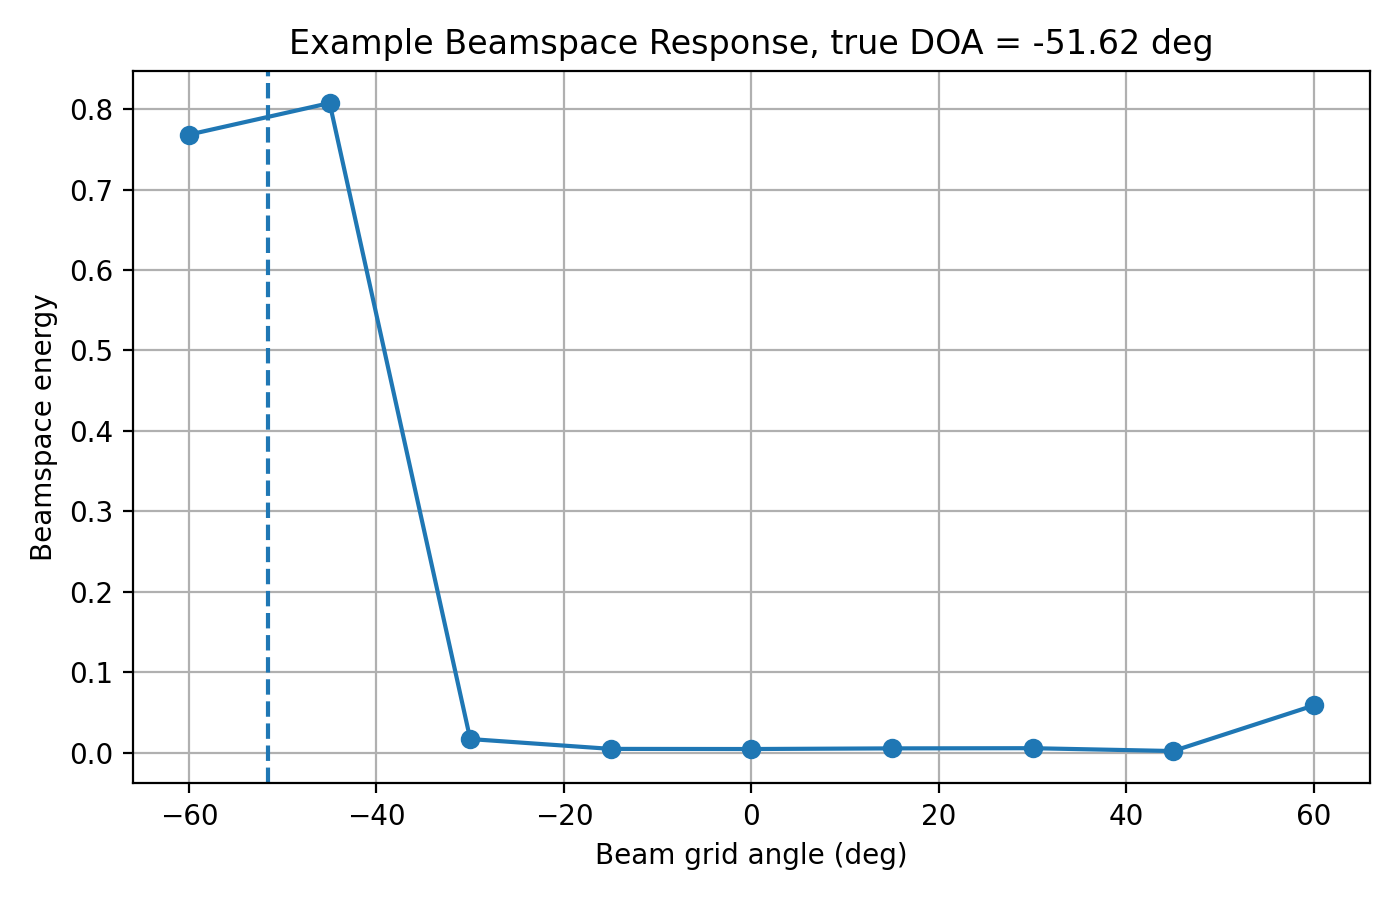
\includegraphics[width=0.80\textwidth]{run_001_example_beamspace_response.png}
\caption{Example beamspace response from the Phase 1 ULA simulation.}
\label{fig:beamspace}
\end{figure}

\section{Nearest-Centroid Baseline}

The non-spiking reference classifier is a nearest-centroid classifier trained on the normalized beamspace features. This classifier is deterministic, interpretable, and lightweight. Its purpose is to establish the amount of DOA-sector information available in the compact feature vector before converting the features into spike trains.

The nearest-centroid baseline achieved
\begin{equation}
    \text{Accuracy}_{\text{baseline}} = 0.869048.
\end{equation}

\begin{table}[H]
\centering
\caption{Nearest-Centroid Accuracy Versus SNR}
\begin{tabular}{rr}
\toprule
SNR (dB) & Accuracy \\
\midrule
-10 & 0.758333 \\
-5 & 0.908333 \\
0 & 0.891667 \\
5 & 0.858333 \\
10 & 0.866667 \\
15 & 0.925000 \\
20 & 0.875000 \\
\bottomrule
\end{tabular}
\end{table}

\section{Spike Encoding and LIF-Inspired Inference}

Normalized beamspace features are converted into binary spike trains using rate-based encoding. A larger normalized feature value corresponds to a higher probability of spike emission across the time window. This representation is sparse and temporal, making it a useful abstraction for later hardware-oriented experiments.

The LIF-inspired classifier is implemented as a class-level leaky membrane accumulator. It is not a biologically detailed SNN. Instead, it is a hardware-facing approximation in which each class accumulates spike-driven evidence over time. The membrane state can be interpreted as
\begin{equation}
    v_c[t] = \alpha v_c[t-1] + i_c[t],
\end{equation}
where $v_c[t]$ is the membrane value for class $c$, $\alpha$ is the leak factor, and $i_c[t]$ is the spike-driven input current at time step $t$.

The fixed Run 003 configuration used
\begin{equation}
    T=20, \qquad \alpha=0.97.
\end{equation}
It achieved
\begin{equation}
    \text{Accuracy}_{\text{LIF, fixed}} = 0.825000,
\end{equation}
with mean stable-decision latency
\begin{equation}
    \bar{L} = 6.423810 \text{ time steps}.
\end{equation}

\section{Accuracy and Latency Analysis}

Run 004 generated report-ready figures comparing the nearest-centroid baseline and the LIF-inspired classifier across the same SNR grid. Figure~\ref{fig:accuracy_comparison} compares accuracy versus SNR. Figure~\ref{fig:latency} shows mean stable-decision latency versus SNR.

\begin{figure}[H]
\centering
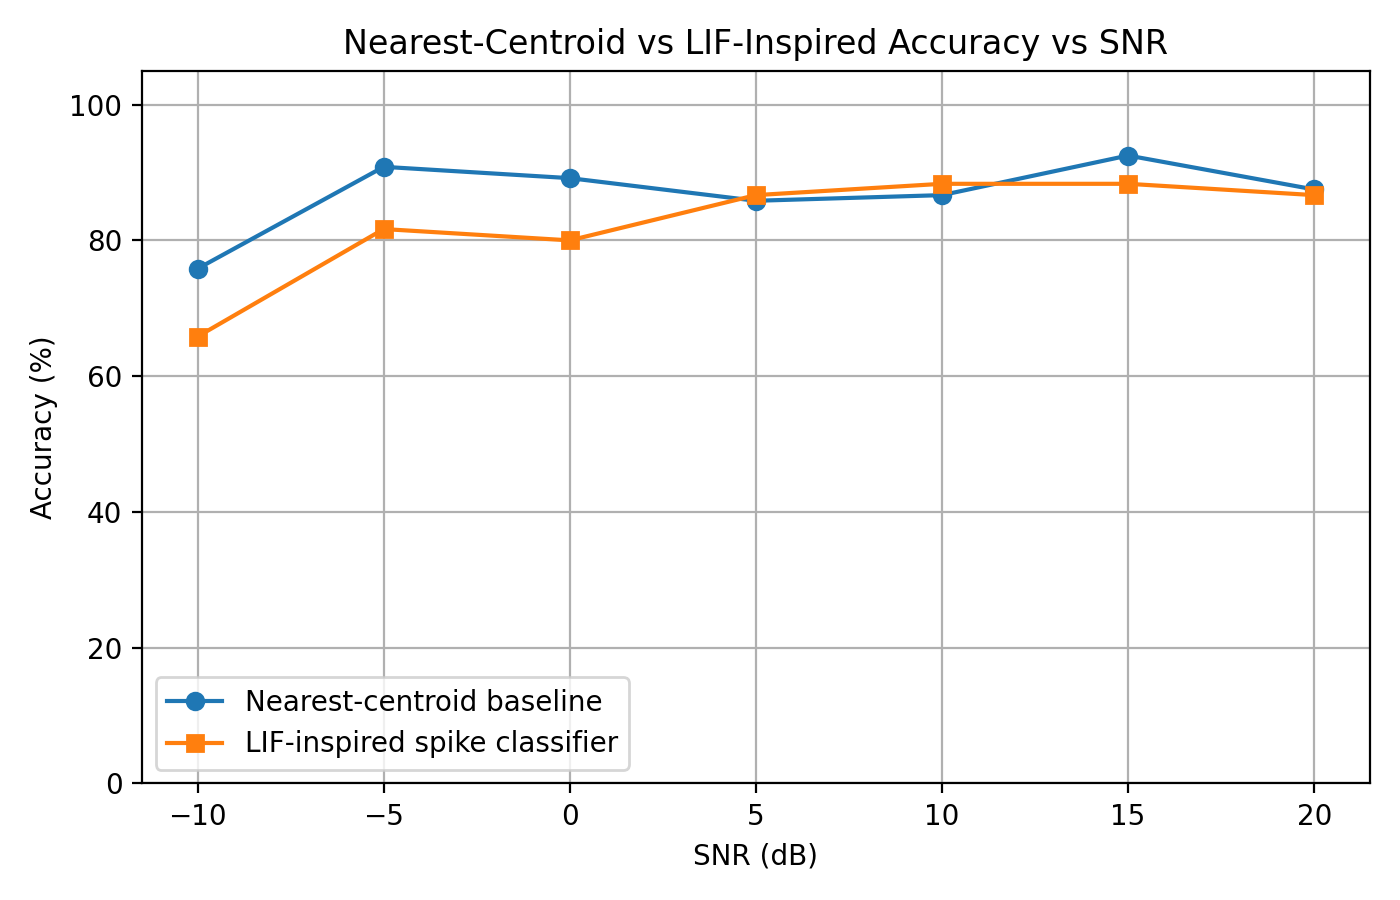
\includegraphics[width=0.82\textwidth]{run_004_accuracy_comparison_vs_snr.png}
\caption{Accuracy comparison between the nearest-centroid baseline and the LIF-inspired classifier.}
\label{fig:accuracy_comparison}
\end{figure}

\begin{figure}[H]
\centering
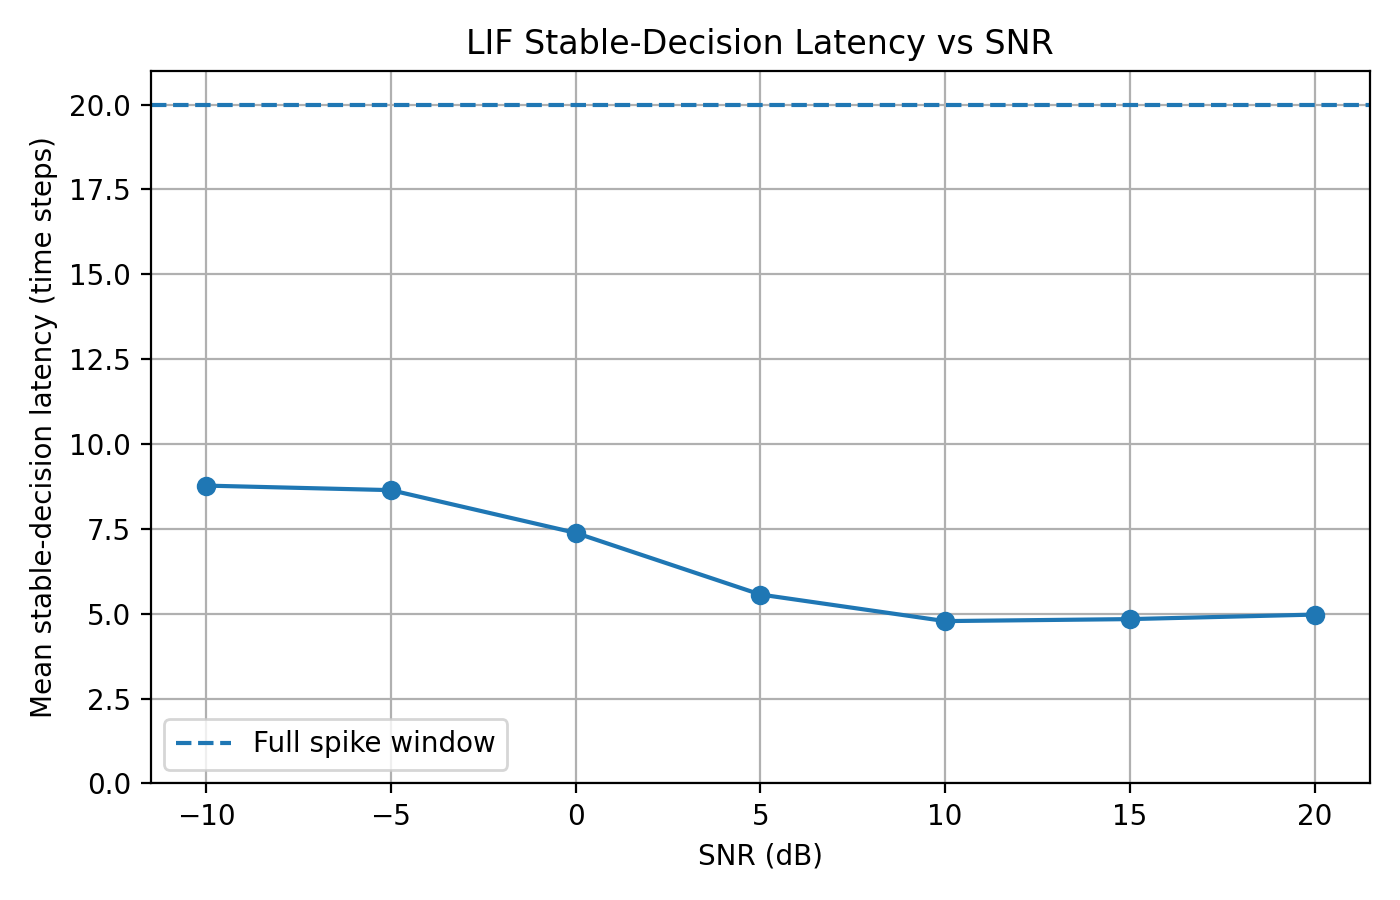
\includegraphics[width=0.82\textwidth]{run_004_lif_latency_vs_snr.png}
\caption{Mean stable-decision latency of the LIF-inspired classifier versus SNR.}
\label{fig:latency}
\end{figure}

The latency trend supports the edge-inference interpretation. When the signal quality is higher, the LIF decision generally stabilizes earlier. This suggests that temporal inference can support early-exit or adaptive-latency decision logic in later embedded implementations.

\section{Run 005 Parameter Sweep}

Run 005 evaluated the sensitivity of the LIF-inspired classifier to spike-window length and membrane leak factor. The sweep grid was
\begin{equation}
    T \in \{10,20,30,40\}, \qquad \alpha \in \{0.90,0.95,0.97,0.99\}.
\end{equation}
This created 16 configurations.

\begin{table}[H]
\centering
\caption{Run 005 Key Results}
\begin{tabular}{lrrrr}
\toprule
Case & $T$ & Leak & Accuracy & Mean latency \\
\midrule
Best LIF accuracy & 40 & 0.99 & 0.841667 & 8.396429 \\
Lowest latency & 10 & 0.99 & 0.776190 & 3.782143 \\
Fixed Run 003 & 20 & 0.97 & 0.825000 & 6.423810 \\
Non-spiking baseline & -- & -- & 0.869048 & -- \\
\bottomrule
\end{tabular}
\end{table}

\begin{table}[H]
\centering
\caption{Full Run 005 LIF Parameter Sweep}
\begin{tabular}{rrrr}
\toprule
$T$ & Leak & Accuracy & Mean latency \\
\midrule
10 & 0.90 & 0.773810 & 4.280952 \\
10 & 0.95 & 0.778571 & 4.011905 \\
10 & 0.97 & 0.779762 & 3.914286 \\
10 & 0.99 & 0.776190 & 3.782143 \\
20 & 0.90 & 0.809524 & 7.732143 \\
20 & 0.95 & 0.816667 & 6.579762 \\
20 & 0.97 & 0.819048 & 6.340476 \\
20 & 0.99 & 0.816667 & 5.753571 \\
30 & 0.90 & 0.802381 & 10.946429 \\
30 & 0.95 & 0.829762 & 8.870238 \\
30 & 0.97 & 0.838095 & 8.126190 \\
30 & 0.99 & 0.832143 & 7.352381 \\
40 & 0.90 & 0.801190 & 14.945238 \\
40 & 0.95 & 0.822619 & 10.778571 \\
40 & 0.97 & 0.830952 & 9.697619 \\
40 & 0.99 & 0.841667 & 8.396429 \\
\bottomrule
\end{tabular}
\end{table}

\begin{figure}[H]
\centering
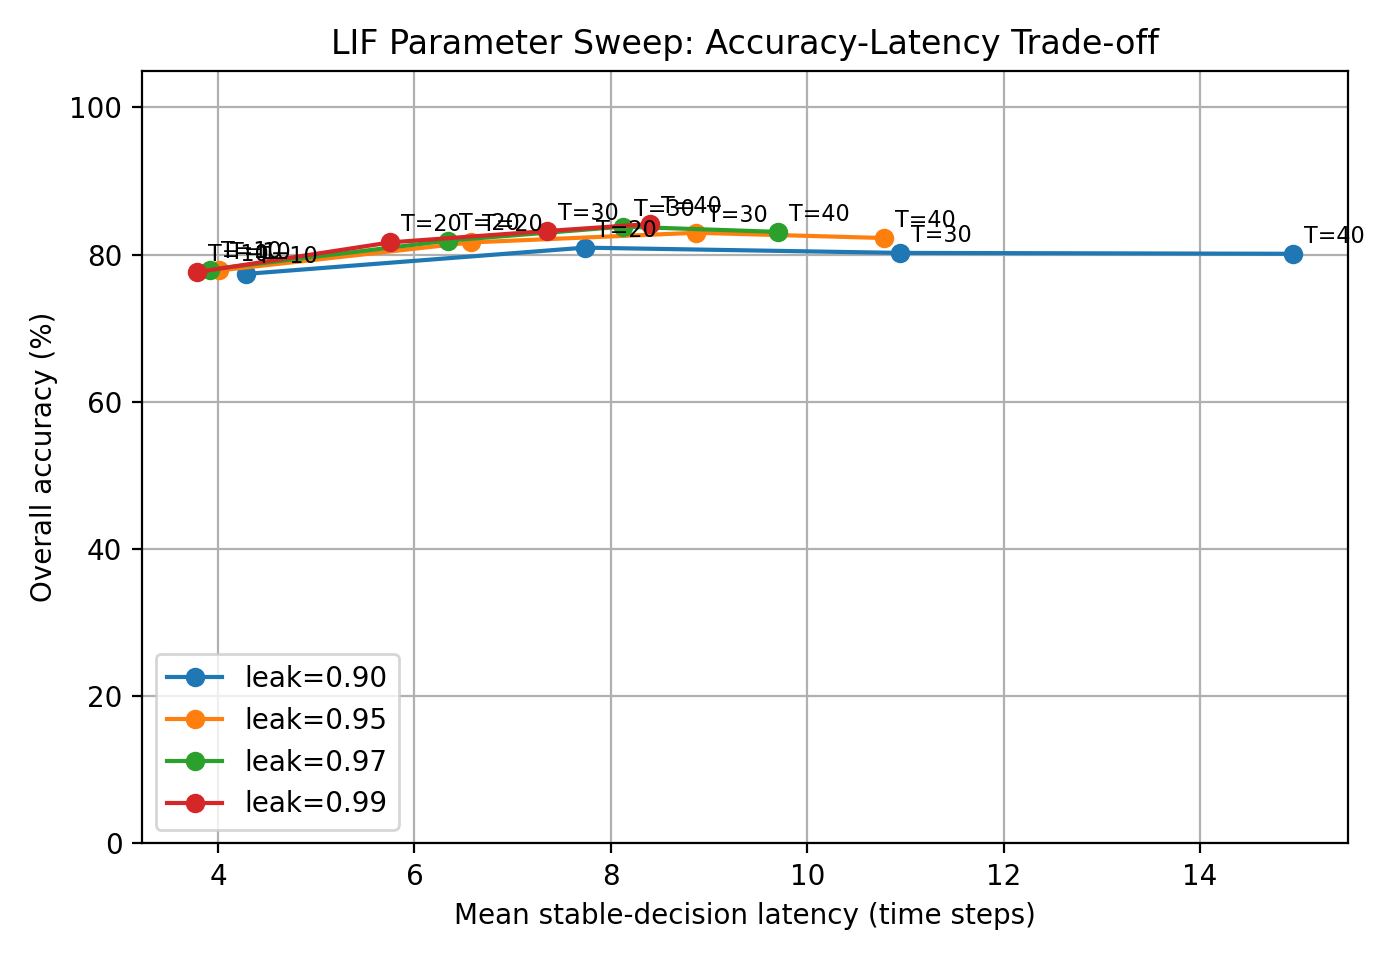
\includegraphics[width=0.82\textwidth]{run_005_lif_accuracy_latency_tradeoff.png}
\caption{Run 005 LIF accuracy--latency trade-off across time-window and leak configurations.}
\label{fig:tradeoff}
\end{figure}

\section{Engineering Interpretation}

The parameter sweep confirms a clear accuracy--latency design trade-off. Increasing the spike time window generally improves classification accuracy because the rate-coded representation has more time steps to approximate the original continuous feature vector. However, a longer time window can increase temporal budget and stable-decision latency.

The leak factor controls evidence retention. Higher leak values preserve accumulated information better. In this prototype, the best LIF accuracy occurs at $T=40$ and leak $=0.99$. The best LIF result improves over the fixed Run 003 configuration but remains below the continuous nearest-centroid baseline. This result is expected and useful: spike-based inference trades some continuous-valued accuracy for sparse temporal processing and explicit latency control.

\section{Conclusion}

The Phase 1 Python prototype successfully establishes an end-to-end DOA-sector inference pipeline based on a physics-derived ULA signal model. The nearest-centroid classifier demonstrates that compact beamspace features provide strong sector-level DOA information, achieving 86.9\% test accuracy.

The LIF-inspired classifier demonstrates that the same normalized features can be converted into sparse temporal spike trains and classified using a hardware-facing leaky evidence accumulator. The fixed LIF configuration achieves 82.5\% accuracy, while the Run 005 parameter sweep improves the best LIF result to 84.17\%.

The Phase 1 result is therefore a valid embedded-AI reference baseline. The natural next step is to convert the Python reference model into a more formal course report and then extend the project toward richer radar/DOA case studies or embedded implementation.

\appendix

\section{Additional Theoretical Details}

\subsection{ULA Steering Vector and Phase Progression}

For a ULA with inter-element spacing $d$, the path-length difference between adjacent sensors is $d\sin\theta$ under the broadside convention. The corresponding phase shift is
\begin{equation}
    \psi(\theta)=kd\sin\theta=\frac{2\pi d}{\lambda}\sin\theta.
\end{equation}
For half-wavelength spacing, $d=\lambda/2$, this becomes
\begin{equation}
    \psi(\theta)=\pi\sin\theta.
\end{equation}
This phase progression is the physical basis for the steering vector used to generate DOA-dependent array snapshots.

\subsection{Beamspace Energy Interpretation}

The beamspace response
\begin{equation}
    p(\phi)=b^{H}(\phi)R_{xx}b(\phi)
\end{equation}
can be interpreted as the output power of a conventional beam steered toward grid angle $\phi$. If the grid steering vector is aligned with the true source direction, the response tends to be larger. Therefore, the vector of grid responses provides a compact angular signature for sector classification.

\subsection{Nearest-Centroid Rule as a Linear Score}

The nearest-centroid decision rule can be expanded as
\begin{align}
    \hat{c}
    &=\arg\min_c \|x-\mu_c\|_2^2 \\
    &=\arg\min_c \left(x^Tx -2\mu_c^Tx + \mu_c^T\mu_c\right).
\end{align}
Since $x^Tx$ does not depend on class, the equivalent decision is
\begin{equation}
    \hat{c}=\arg\max_c \left(2\mu_c^Tx-\|\mu_c\|_2^2\right).
\end{equation}
This form is useful for the LIF-inspired implementation because it can be interpreted as class evidence accumulation using class-dependent weights and biases.

\subsection{Spike Encoding Statistics}

For rate-based encoding, the spike count for feature $i$ over $T$ time steps is
\begin{equation}
    K_i=\sum_{t=1}^{T}s_i[t].
\end{equation}
If $s_i[t]\sim \mathrm{Bernoulli}(z_i)$, then
\begin{equation}
    \mathbb{E}[K_i]=Tz_i,
\end{equation}
\begin{equation}
    \mathrm{Var}(K_i)=Tz_i(1-z_i).
\end{equation}
Therefore, a longer spike window reduces relative stochastic error but increases the temporal budget.

\subsection{LIF Leak and Latency Interpretation}

The LIF-inspired update
\begin{equation}
    v_c[t]=\alpha v_c[t-1]+i_c[t]
\end{equation}
acts as a leaky temporal integration of evidence. When $\alpha$ is close to one, previous evidence is retained for more time steps. When $\alpha$ is smaller, the classifier reacts more strongly to recent spikes but may lose accumulated evidence more quickly. This explains why the Phase 1 parameter sweep uses both $T$ and $\alpha$ as design variables.

\section*{References}
\addcontentsline{toc}{section}{References}

\begin{thebibliography}{9}
\bibitem{vanTrees}
H. L. Van Trees, \emph{Optimum Array Processing}. Wiley, 2002.

\bibitem{haykin}
S. Haykin, \emph{Adaptive Filter Theory}. Pearson, 2014.

\bibitem{roy}
K. Roy, A. Jaiswal, and P. Panda, ``Towards spike-based machine intelligence with neuromorphic computing,'' \emph{Nature}, vol. 575, pp. 607--617, 2019.

\bibitem{maass}
W. Maass, ``Networks of spiking neurons: The third generation of neural network models,'' \emph{Neural Networks}, vol. 10, no. 9, pp. 1659--1671, 1997.
\end{thebibliography}

\end{document}
